The standard model of particle physics (SM) describes the fundamental particles and interactions between them. It is a theory that successfully predicted the existence of several particles and has been tested extensively, \eg in electroweak precision measurements at LEP. \\
Although the SM is a successful theory, there are also open questions which can not be answered within the SM. Thus, several theories have been developed to address problems which go beyond the SM. One of such extensions is supersymmetry (SUSY) for which, however, no experimental evidence has been found so far. \\
After a short introduction to the phenomenology of the standard model, including a discussion of specific shortcomings, the basic concepts of supersymmetry are introduced in this chapter. In addition, general concepts of searches for supersymmetry at collider experiments are discussed together with a summary of the current status of the results of such searches which have been performed in the past.
\section{The Standard Model of Particle Physics}
\label{sec:sm}
The SM comprises the elementary particles and their interactions~\cite{Agashe:2014kda}. In general, one distinguishes between two types of particles: fermions and bosons. While matter particles are fermions with half-integer spin, the fundamental forces are mediated via bosons, carrying integer spin. An overview of the contents of the SM is given in Fig.~\ref{fig:SM} in which the particles are denoted together with their interactions.\footnote{Gravity is not included in the standard model and thus it is not discussed in this thesis.} 
\begin{figure}[!tp]
  \centering 
  \begin{tabular}{c}
    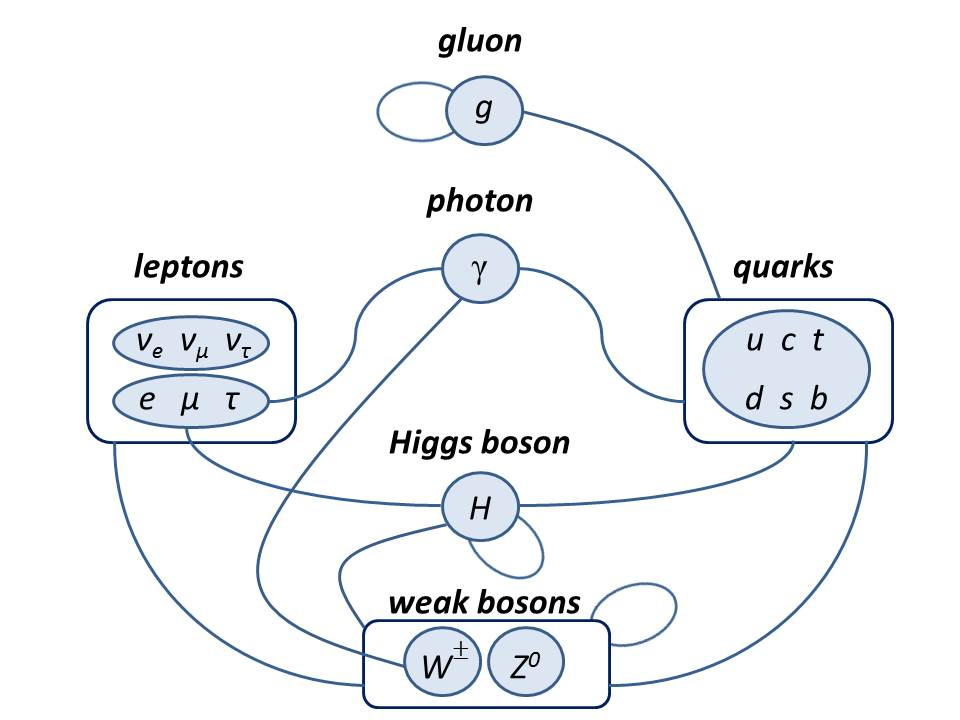
\includegraphics[width=0.9\textwidth]{figures/SM.jpg}
  \end{tabular}
  \caption{Overview of particles contained in the standard model. Blue lines indicate interactions between different particles.}
  \label{fig:SM}
\end{figure}
\\
Mathematically, the standard model is a quantum field theory where interactions between particles are described via gauge symmetries. The underlying gauge group of the standard model is 
\begin{equation*}
SU(3)_{C} \otimes SU(2)_{L} \otimes U(1)_{Y} \; ,
\end{equation*}
where $SU(3)$ is the gauge group of the strong force, and $C$ indicates that this force acts on the colour charge, $SU(2)$ represents the weak force and $L$ denotes that this force only acts on left-handed fermions, while $U(1)$ represents the electromagnetic force acting on the hypercharge $Y$.\\
A brief description of the properties of the particles contained in the SM and the corresponding interactions is given in the following:
\begin{description}

\item \textbf{Matter Constituents:}
In the SM, one distinguishes between twelve different fermions being the elementary constituents of matter. For each fermion there exists also an antiparticle which carries the opposite signed quantum numbers.
 \begin{description}
  \item \textit{Leptons:} The SM contains, in total, six leptons, which are three negatively charged leptons (\lel, \lmu, \ltau) and three neutral leptons (\nue, \numu, \nutau), the neutrinos. In addition to the charge, leptons are also distinguished according to the lepton numbers which are electron number $L_{\lel} = 1$ for electron and electron-neutrino, muon number $L_{\lmu} = 1$ for muon and muon-neutrino and tauon number $L_{\ltau} = 1$ for tauon and tauon-neutrino. Each pair of lepton and neutrino carrying the same lepton number is arranged in a so-called \textit{generation} where \lel and \nue belong to the first generation, \lmu and \numu to the second and \ltau and \nutau to the third, respectively.
  \item \textit{Quarks:} The remaining six fermions in the SM are quarks and can be grouped into generations analogous to the leptons. The first generation comprises the up- and down-quark (\qu, \qd), the second the charm- and strange-quark (\qc, \qs) and the third the top- and bottom-quark (\qt, \qb). All quarks carry electrical charge, but in contrast to leptons, it is not integer, but $+2/3$ for the up-type quarks (\qu, \qc, \qt) and $-1/3$ for down-type quarks (\qd, \qs, \qb). Besides to the electrical charge, quarks also carry colour charge which comes in three types.
 \end{description}
In addition to the attributes described above, fermions are furthermore characterized by the weak isospin. In each generation, left-handed fermions form an isospin-doublet with a weak isospin of $\pm 1/2$ while right-handed components are isospin-singlets with a weak isospin of 0. 
\item \textbf{Fundamental Forces:}
Matter particles interact with each other through fundamental forces mediated via gauge bosons. These bosons arise from the principle of local gauge invariance under symmetry transformations. 
 \begin{description}
  \item \textit{Electromagnetic Force:} The description of the electromagnetic force is based on the theory of \textit{Quantum Electrodynamics} (QED). It is exchanged between electrically charged particles, like the charged leptons and quarks, by the exchange of photons. These are massless and electrically neutral resulting in the property that the electromagnetic force is long ranged.
  \item \textit{Weak Force:} The weak force acts on left-handed fermions, \ie on fermions with non-zero weak isospin, and manifests in charged and neutral currents. Weak interactions preferably take place within one fermion generation. However, since the mass eigenstates in the weak interaction differ from the flavour eigenstates, also transitions between different generations are possible. In the quark-sector typically a representation is chosen where the up-type flavour eigenstates correspond to the mass eigenstates and the down-type quarks mix. This mixing is described by the CKM-matrix ~\cite{PhysRevLett.10.531, PTP.49.652}. This is a unitary matrix, described by three mixing angles and one CP-violating phase, which indicates the relative strength between individual transitions. Similarly, also in the neutrino sector a mixing between the weak and the mass eigenstates occurs which leads to the phenomenom of \textit{neutrino oscillation}~\cite{Maki:1962mu, Pontecorvo:1967fh, Fukuda:1998mi}.
  \item \textit{Strong Force:} The theoretical framework describing the strong force is called Quantum Chromodynamics (QCD). It is mediated via eight massless gluons and acts on the colour charge which is carried for instance by quarks. In contrast to the photon, which is electrically neutral and thus can not interact with itself, gluons carry a colour charge and hence couple to themselves. The colour charge exists in three different states commonly denoted as 'red', 'green' and 'blue'. \\
Regarding the dependence on the distance, the strong force behaves differently than other fundamental forces: the coupling strength increases with rising distance. This is a consequence of the different colour states and the self-coupling property of gluons. It is referred to as \textit{confinement}~\cite{Alkofer:2006fu} and describes the fact that coloured objects can not exist freely. Actually, when separated, coloured objects start to build new coloured particles until only a colour neutral formation is left. Such colourless objects linked by the strong force are named \textit{hadrons}. On the other hand, particles taking part in the strong interaction start to behave quasi-free, \ie the coupling strength is small, when the distance decreases. This feature is known as \textit{asymptotic freedom}~\cite{PhysRevLett.30.1346, PhysRevLett.30.1343}. \\
A typical example for a hadron is the proton. In a simplified picture, it is composed of three quarks: two up quarks and one down quark (\textit{valence quarks}). However, the valence quarks continuously exchange gluons which can exchange further gluons or split into quark-antiquark pairs (\textit{sea quarks}). The constituents of the proton are commonly denoted \textit{partons} and the internal proton structure is described by \textit{parton-distribution functions} (PDFs) specifying the momentum fraction of the proton carried by individual partons.
 \end{description}
First proposed by Salam, Glashow and Weinberg~\cite{Glashow:1961tr, Weinberg:1967tq}, the electromagnetic and the weak force could be successfully unified into the electroweak force. As denoted earlier, the weak force acts on the weak isospin $T_{3}$ while the electromagnetic force acts on the hypercharge $Y$. These two quantities are connected via the following relation to the electric charge $Q$
\begin{equation*}
Q = T_{3} + Y/2
\end{equation*}
In the electroweak theory, three gauge bosons $W^{1,2,3}_{\mu}$ are introduced for $SU(2)_{L}$ and one gauge boson $B_{\mu}$ for $U(1)_{Y}$. The physical states photon, \Wpm and \Z boson are formed by mixing of these massless states. While the charged $\Wpm$ bosons are superpositions of $W^{1}_{\mu}$ and $W^{2}_{\mu}$, the fields $A_{\mu}$ of the photon and $Z_{\mu}$ of the neutral vector boson are obtained by a mixing of the gauge fields $W^{3}_{\mu}$ and $B_{\mu}$ according to
\begin{equation}
\left(
\begin{matrix}
A_{\mu} \\ Z_{\mu}
\end{matrix}
\right)
=
\left(
\begin{matrix}
\mathrm{cos} \, \theta_{W} & \mathrm{sin} \, \theta_{W} \\
-\mathrm{sin} \, \theta_{W} & \mathrm{cos} \, \theta_{W}
\end{matrix}
\right)
\left(
\begin{matrix}
 B_{\mu} \\ W^{3}_{\mu} 
\end{matrix}
\right)
\end{equation}
with the weak mixing angle $\theta_{W}$. This mixing angle relates also the electromagnetic coupling strength $e$ and the weak coupling strength $g$ according to
\begin{equation}
e = g \, \mathrm{sin} \, \theta_{W} \; .
\end{equation}
The fields $W^{\mu}$ couple only to left-handed fermions, such that the same holds also for $W^{\pm}$. Since however, the $B^{\mu}$ couples to left- and right-handed states, a coupling to left- and right-handed fermions takes place for $\gamma$ and $Z^0$ as well. Unlike the photon, the $W^{\pm}$ and $Z$ vector bosons are massive with masses\footnote{In this thesis, natural units are used, \ie $\hbar = c =1$. Thus, also particle masses and momenta have the dimension of energies.} of $\Wpm = 80.385 \pm 0.015$\gev and $\Z = 91.1876 \pm 0.0021$\gev~\cite{Agashe:2014kda}. As a result, the weak interaction is suppressed with respect to the electromagnetic force. 
\item \textbf{Higgs Boson:} The electroweak theory in the current representation requires that fermions and bosons are massless particles as mass terms violate the gauge invariance under $SU(2)_{L} \otimes U(1)_{Y}$ transformations. This is in contradiction to experimental observations which have shown that all particles, except for photon and gluon, in fact do have mass. \\
An explanation for the generation of particle masses without violation of the principles of the electroweak theory is provided by the \textit{Higgs-mechanism}~\cite{PhysRevLett.13.508, PhysRevLett.13.321, PhysRevLett.13.585} which is based on the concept of spontaneous symmetry breaking. The main idea behind this meachnism is that while in general the principle of local gauge invariance is obeyed, it is explicitly broken by the ground state. \\
In the context of the Higgs-mechanism, this is realized by the introduction of the Higgs field $\Phi$ described by a potential 
\begin{equation*}
\mathcal{V}(\Phi) = \mu^2 \Phi^+\Phi^- \, + \, \lambda (\Phi^+\Phi^-)^2
\end{equation*}
with parameters $\mu$ and $\lambda$. Choosing $\mu^2$ to be negative and $\lambda$ positive, the potential has a non-zero minimum value with the vacuum expectation value
\begin{equation*}
v = \sqrt{\frac{-\mu^2}{2\lambda}} \; .
\end{equation*}
Expansion of the Higgs field around this vacuum expectation value eventually leads to a new spin 0 particle, the scalar \textit{Higgs boson} which is a quantum excitation of one of the components of the Higgs field. Furthermore, the masses of gauge bosons are generated by the couplings to the Higgs field according to
\begin{equation*}
m_{\gamma} = 0, \;\;\; m_W = \frac{v}{2}g, \;\;\; m_Z = \frac{m_W}{\mathrm{cos}\theta_{W}}, \;\;\; m_H = \sqrt{-2\mu^2} \;.
\end{equation*}
Similarly, the Higgs mechanism introduces mass terms for fermions 
\begin{equation*}
m_{f} = G \frac{v}{\sqrt{2}}
\end{equation*}
resulting from Yukawa couplings to the Higgs field with coupling constants $G_i$. \\
The discovery of a new boson at a mass of around 125~\gev has been announced by the ATLAS and CMS collaborations in 2012~\cite{Aad:2012tfa, Chatrchyan:2012ufa}. As all properties of this new boson are consistent with SM predictions for the Higgs boson so far (\cf for instance~\cite{Aad:2013wqa, Aad:2014eva, Aad:2014eha, CMS-PAS-HIG-14-009}), this indicates that the last remaining gap of the SM could finally be closed.   
\end{description}

\subsection{Limitations of the Standard Model}
\label{subsec:sm_shortcomings}
Although the SM has been very successful so far leading to several discoveries while withstanding numerous precision tests, it is known to be an incomplete theory. Some of the shortcomings of the SM are:
\begin{description}
\item \textbf{Gravity:} As stated already earlier, the SM contains no description of gravity. In particular, it is currently not possible to unify general relativity and quantum theory in one common concept.
\item \textbf{Matter antimatter asymmetry:} According to the SM, matter and anitmatter exist to equal amounts in the universe, which is in fact not the case. A theory which would be able to explain the observed asymmetry needs some source of $CP$-violation. The only source of $CP$-violation within the SM is arising from the CKM matrix as described in~\ref{sec:sm}. However, this is not enough to be able to explain the degree of matter-antimatter asymmetry in the universe~\cite{bib:CPViolation}.    
\item \textbf{Unification of couplings:} The unification of the electromagnetic and the weak force leads to the question if it is possible to further unify the electroweak force with the strong force, in order to build a combined theory, usually referred to as Grand Unified Theory (GUT). This would require that the coupling constants of the SM intersect when extrapolating them from the electroweak to the GUT scale. However, this feature is not observed within the SM.
\item \textbf{Nature of dark matter:} There exist several cosmological observations that indicate that the matter described by the SM makes up only $4.9$\% of the universe~\cite{Ade:2013zuv}. A by far larger part of $26.8$\% is assigned to so-called \textit{dark matter} which is presumably neutral and only weakly interacting. The only particles within the SM possessing such attributes are neutrinos. However, they are not able to account for the whole relic density present in the universe~\cite{Bertone:2004pz}. 
\item \textbf{Hierarchy problem:} The observable mass of the Higgs boson is given by the bare mass of the Higgs boson plus contributions arising from higher order corrections caused by each massive SM particle. For a fermion with mass $m_f$ and Yukawa coupling $\lambda_f$ to the Higgs field, the corrections to $m_H^2$ are
\begin{equation}
\label{eq:hierarchy}
\Delta m_H^2 \propto -\frac{|\lambda_f|^2}{8\pi^2}\Lambda_\mathrm{UV}^2 \propto m_f^2
\end{equation}
 where $\Lambda_\mathrm{UV}$ is an ultraviolet cut-off scale. Typically, this cut-off scale is interpreted as the energy at which new physics enter. If it is chosen to be the Planck scale, the Higgs mass is several orders of magnitudes larger than the electroweak scale and thus, would require an enormous amount of fine-tuning at each order of perturbation theory to yield the expected Higgs mass around $\mathcal{O}(100)$\gev. 
\end{description} 

\section{Supersymmetry}
\label{sec:susy}
In order to overcome the weaknesses of the SM and to provide explanations for so far unsolved problems, several theories have been developed which go beyond the SM. Among those, a favoured extension is \textit{supersymmetry} (SUSY), as it is able to provide several benefits at once. The first supersymmetric four-dimensional quantum field theory has been introduced by Wess and Zumino in 1974~\cite{bib:WessZumino}. \\
In this section, a brief introduction to the general concept of supersymmetry is given with focus on the \textit{Minimal Supersymmetric Standard Model} (MSSM). For detailed reviews see, \eg\cite{Aitchison:2005cf, Martin:1997ns}.\\ 
\\
%The basic idea behind supersymmetry is that each standard model particle gets a supersymmetric partner particle which possesses the same quantum numbers except for the spin which differs by $1/2$. 
The basic idea of a supersymmetric theory is that a fermionic state is converted into a bosonic state and vice versa by the generator of a supersymmetry transformation $Q$ according to
\begin{equation*}
Q \ket{\mathrm{fermion}} \, = \, Q \ket{\mathrm{boson}}, \hspace{20mm} Q \ket{\mathrm{boson}} \, = \, Q \ket{\mathrm{fermion}}.
\end{equation*}
The supersymmetric fermionic and bosonic partner particles are called \textit{superpartners} and form together the irreducible representations of the supersymmetry algebra named \textit{supermultiplets} with the same number of fermionic and bosonic degrees of freedom. In case of unbroken supersymmetry, partner particles within one supermultiplet have the same mass as well as the same quantum numbers like electric charge, weak isospin and colour degrees of freedom, except for the spin. Commonly, supersymmetric particles are denoted \textit{sparticles}. \\
\\
In a general supersymmetric theory fulfilling the criteria of gauge invariance and renormalisability, processes are allowed which violate either lepton or baryon number conservation. However, a baryon and lepton number violation would imply for instance a rapid decay of protons. The lower limit on the proton lifetime is found to be $5.9 \times 10^{33}$ years at 90\% confidence level~\cite{PhysRevD.90.072005} and indicates that such processes must be suppressed. In order to achieve this, a new quantum number called \textit{R-parity} is introduced according to  
\begin{equation*}
R = (-1)^{3(B-L) + 2S}
\end{equation*}
with baryon number $B$, lepton number $L$ and spin $S$. It is a multiplicative quantum number and amounts to $R= +1$ for SM particles while it is $R = -1$ for supersymmetric particles. Assuming $R$-parity conservation no baryon or lepton number violation processes occur.\footnote{There exist also several $R$-parity violating SUSY models which are not in contradiction to the observed proton lifetime (\cf, \eg~\cite{Martin:1997ns}). However, these are not subject of this thesis and thus not discussed.} In addition, the assumption of $R$-parity conservation leads to further phenomenological implications:
\begin{itemize}
\item SUSY particles can only be produced in pairs at collider experiments as only even numbers of supersymmetric particles can occur at an interaction vertex.
\item The lightest supersymmetric particle (LSP) is stable and thus any decay chain of a supersymmetric particle finally ends in a state containing an odd number of LSPs.
\end{itemize}
A $R$-parity conserving supersymmetric theory provides some elegant solutions to open questions, as raised in Sec.~\ref{subsec:sm_shortcomings}:
\begin{itemize}
 \item The Higgs mass suffers from quadratically divergent contributions arising from higher-order corrections caused by SM particles. However, since in SUSY each SM particle gets a supersymmetric partner, these higher order corrections cancel. For instance for the fermion contributions described in Eq.~\ref{eq:hierarchy}, the quadratically divergent terms are canceled by contributions with opposite sign that arise from a scalar with same mass and thus the same coupling strength to the Higgs field. Since the same cancelation occurs for bosons vice versa, SUSY is able to provide a solution to the hierarchy problem. However, no observation of such kind of supersymmetric particles with exact same masses as their SM correpondents has been made, such that supersymmetry in fact has to be a broken symmetry. In order to still be able to provide a solution to the hierarchy problem, supersymmetric particles are expected to be not heavier than $\mathcal{O}(\mathrm{1\tev})$, which is typically referred to as \textit{natural supersymmetry}. This is the main argument why one would expect masses of supersymmetric particles to be in the TeV range, well within the reach of the LHC. Some more considerations about natural SUSY follow in Sec.~\ref{subsec:natural_susy}.
 \item Considering the existence of low scale supersymmetric particles, the coupling constants of the forces meet in one point when extrapolating the couplings from the electroweak to the GUT scale. This effect is illustrated in Fig.~\ref{fig:couplings}. It is visible that the evolution of the couplings is modified with respect to the SM at that energy scale where the supersymmetric particles enter. In general, this hints to the possibility of a grand unification.
\begin{figure}[!t]
  \centering
  \begin{tabular}{c}
    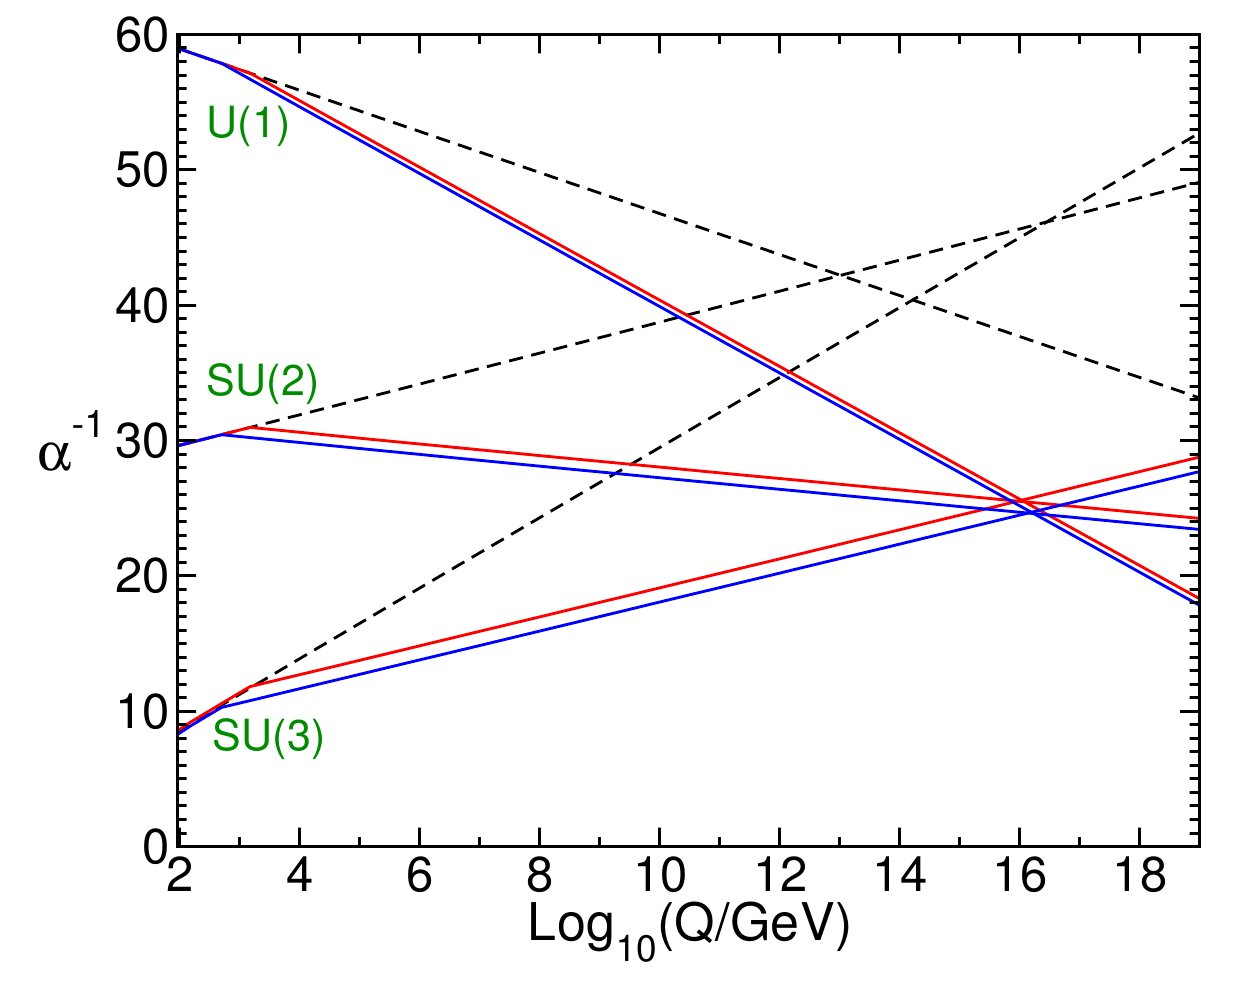
\includegraphics[width=0.55\textwidth]{figures/Couplings.jpg}
  \end{tabular}
  \caption{Comparison of the renormalization group evolution of the couplings $\alpha_{a}^{-1}$ in the SM (dashed lines) and the MSSM (solid lines) including two-loop effects. The masses of the supersymmetric particles in the MSSM are considered as a common threshold changing between 500\gev and 1.5\tev while the strong coupling constant $\alpha_{3}(m_{Z})$ is varied between 0.117 and 0.121. Taken from~\cite{Martin:1997ns}.}
  \label{fig:couplings}
\end{figure}
 \item $R$-parity conserving SUSY models provide a suitable dark matter candidate. As discussed previously, each decay of supersymmetric particles finally leads to the existence of an LSP which is stable. Thus, it is an adequate DM candidate when it is only weakly interacting.
 \item Supersymmetry is in principal also suited to explain the observed matter-antimatter asymmetry in the universe, as especially, the description of supersymmetry breaking can involve $CP$-violating phases. However, these phases are strongly constraint by experimental results (\cf for instance~\cite{Ibrahim:2007fb} for a comprehensive review).
 \item SUSY might also provide an indication of the nature of gravity. As denoted in Sec.~\ref{subsec:sm_shortcomings}, it is currently not possible to unify general relativity and quantum theory. However, supersymmetry is a crucial requirement for \textit{string theories} which are the only suited candidates for a quantum field theory of gravity to date (see, \eg\cite{RevModPhys.47.123}). 
\end{itemize} 

\subsection{Natural Supersymmetry}
\label{subsec:natural_susy}
As introduced above, SUSY models are considered natural, if they provide a solution to the hierarchy problem. Commonly, certain measures are introduced to estimate the naturalness of a supersymmetric model. \\
One example is the Veltman definition of naturalness~\cite{veltman1981infrared}. This states that radiative contributions should not exceed tree-level effects in size, regarding the mass of a scalar particle. Another definition is given by Babieri and Giudice~\cite{Barbieri198863} which do not restrict the magnitude of the radiative corrections, but the sensitivity of the physical mass of a scalar $m$ to small changes in the bare couplings $\lambda_0$. This constraint is often imposed by quantifying the amount of necessary fine-tuning $\Delta$ according to
\begin{equation}
\left| \frac{\lambda_0}{m^2}\frac{\partial m^2}{\partial \lambda_0} \right| < \Delta \; .
\end{equation}
While the value of $\Delta$ has been set to $\sim10$ in the past, it increased over the years such that also values of $\sim100$ or even $\sim1000$ are considered as reasonable values~\cite{Craig:2013cxa}. \\
Such conditions can be used in order to derive constraints on the spectrum of superpartners which regulate the hierarchy problem. Here, it turns out that not all sparticles are equally important and thus, not all have to be situated at the same mass scale. Some typical mass ranges for sparticles considered as natural are given in Sec.~\ref{subsec:mssm}. 

\subsection{The MSSM}
\label{subsec:mssm}
In general, it is possible to have theories with more than one supersymmetry transformation $N$. However, the smallest possible supersymmetric extension of the SM including the full particle spectrum and interactions, \ie a $N = 1$ supersymmetry, is realised in the MSSM. An overview of the respective particle content is given in Tab.~\ref{tab:particle_content}. 
\begin{table}[!t] 
  \centering
%   \makebox[\linewidth]{
    \begin{tabular}{cccc}
%      \hline
      \toprule
      Type & Spin & Gauge eigenstates & Mass eigenstates \\
      \midrule
      \midrule
      Higgs bosons & 0 & $H_{u}^{0}$ $H_{d}^{0}$ $H_{u}^{+}$ $H_{d}^{-}$ & $h^{0}$ $H^{0}$ $A^{0}$ $H^{\pm}$  \\
      \midrule
      & & $\tilde{u}_{L}$ $\tilde{u}_{R}$ $\tilde{d}_{L}$ $\tilde{d}_{R}$ &  see left \\
      Squarks & 0 & $\tilde{s}_{L}$ $\tilde{s}_{R}$ $\tilde{c}_{L}$ $\tilde{c}_{R}$  & see left \\
      & & $\tilde{t}_{L}$ $\tilde{t}_{R}$ $\tilde{b}_{L}$ $\tilde{b}_{R}$ & $\tilde{t}_{1}$ $\tilde{t}_{2}$ $\tilde{b}_{1}$ $\tilde{b}_{2}$ \\
      \midrule
      & & $\tilde{e}_{L}$ $\tilde{e}_{R}$ $\tilde{\nu}_{e}$ &  see left \\
      Sleptons  & 0 & $\tilde{\mu}_{L}$ $\tilde{\mu}_{R}$ $\tilde{\nu}_{\mu}$ & see left \\
      & & $\tilde{\tau}_{L}$ $\tilde{\tau}_{R}$ $\tilde{\nu}_{\tau}$ & $\tilde{\tau_{1}}$ $\tilde{\tau_{2}}$ $\tilde{\nu_{\tau}}$ \\
      \midrule
      Neutralinos  & 1/2 & $\tilde{B}^{0}$ $\tilde{W}^{0}$ $\tilde{H}_{u}^{0}$ $\tilde{H}_{d}^{0}$ & $\tilde{\chi}_{1}^{0}$ $\tilde{\chi}_{2}^{0}$ $\tilde{\chi}_{3}^{0}$ $\tilde{\chi}_{4}^{0}$ \\
      \midrule
      Charginos & 1/2 & $\tilde{W}^{\pm}$ $\tilde{H}_{u}^{+}$ $\tilde{H}_{d}^{-}$ & $\tilde{\chi}_{1}^{\pm}$ $\tilde{\chi}_{2}^{\pm}$ \\
      \midrule
      Gluino & 1/2 & $\tilde{g}$ & see left \\
      \midrule
      Gravitino & 3/2 & $\tilde{G}$ & see left \\
      \bottomrule
    \end{tabular}%}
 \caption{Supersymmetric particles contained in the MSSM neglecting mixing in the first two sfermion generations. Adapted from~\cite{Martin:1997ns}.} 
  \label{tab:particle_content}
\end{table}
This extension is minimal in the sense that it introduces the least feasible number of additional particles to the existing SM particles meaning that each SM fermion gets one superpartner. The interactions and couplings of the supersymmetric particles are the same as for the SM counterparts. The different transformation of left- and right-handed fermions under the gauge groups implies the necessity to introduce separate superpartners for left- and right-handed states as well. These are arranged with their bosonic (spin 0) superpartner in a \textit{chiral} supermultiplet. The labels indicating the left- and right-handed states refer to the helicity of the respective SM particle. These supersymmetric partners of fermions are named \textit{sfermions} distinguishing between \textit{sleptons} and \textit{squarks}, the supersymmetric partners of leptons and quarks. In a similar manner, the SM gauge bosons are arranged in \textit{gauge} supermultiplets together with their fermionic (spin 1/2) supersymmetric correspondents. The SUSY partners of the gauge bosons are named \textit{gauginos} so that the superpartners in the gauge supermultiplets are the \textit{gluino}, \textit{wino} and \textit{bino}. The corresponding gaugino mixtures of the neutral wino and the bino are the \textit{photino} and the \textit{zino}. Furthermore, the supersymmetric particle spectrum is extended by another supermultiplet containing the graviton (spin 2) and the respective supersymmetric partner -- the \textit{gravitino} (spin 3/2). \\
As described in Sec.~\ref{sec:sm}, masses arise in the SM from the concept of spontaneous symmetry breaking implying the existence of the Higgs boson. The supersymmetric partner of the Higgs boson is named \textit{higgsino}. While in the SM one Higgs doublet is sufficient to give mass to all particles, the Higgs sector needs to be extended in the MSSM. Here, two Higgs doublets are needed where one doublet $H_u$ gives mass to the up-type quarks and the other one $H_d$ to the down-type quarks, respectively. These two doublets have together eight degrees of freedom of which three are needed to give mass to the gauge bosons of the weak interaction as in the SM. This results in five physical Higgs bosons which are the two scalar Higgs particles $h^0, H^0$, the pseudoscalar $A^0$ as well as the charged Higgs bosons $H^{\pm}$. As further consequence, there are two vacuum expectation values $v_u$ and $v_d$ present, each assigned to one Higgs doublet, whose ratio $\mathrm{tan} \, \beta = v_u/v_d$ is a free parameter of the model. Within the MSSM the mass of the lightest Higgs boson is restricted to be smaller than the $Z$-boson mass at tree level. However, due to radiative corrections, which mainly arise from the top sector, this limit is enhanced and results in an upper bound of~\cite{Martin:1997ns} 
\begin{equation*}
m_{h^0} \lesssim 135 \gev \; .
\end{equation*}
Consequently, significant contributions from the top squark mass are required to push the mass of the lightest Higgs boson up to a value of around 125\gev. This is somewhat in tension to the requirement of having a stop quark mass close to the top mass in order to solve the hierarchy problem. However, it is still possible to accommodate a Higgs mass of 125\gev without the necessity to decouple the top squark or add new dynamics to the MSSM. These scenarios are referred to as \textit{maximal mixing}~\cite{Djouadi:2005gj}. \\
Similar to the SM, the gauge eigenstates of the SUSY theory are not necessarily equal to the mass eigenstates. A mixing occurs especially in the gaugino sector. Here, the neutral components of the bino and wino mix with the neutral higgsinos and form four mass eigenstates called \textit{neutralinos} $\tilde{\chi}^0$. Similarly, also the charged gauginos and higgsinos mix to the four \textit{charginos} $\tilde{\chi}^{\pm}$. Furthermore, mixing can also appear in the third squark and slepton generation. The mixing is supposed to be significant only for fermions of the third generation as the off-diagonal elements of the sfermion mass matrix are proportional to the mass of the respective SM partner. \\
In order to obtain a natural realization of the MSSM, it is important that certain particles have a particular mass scale~\cite{Craig:2013cxa}. Especially the superpartner of the top quark is expected to be not too heavy, in order to be able to cancel the contributions from top loops to the Higgs mass. These give typically the largest contributions, since the top quark is the heaviest particle in the SM. Assuming a maximal accepted fine-tuning of $\Delta \lesssim 10$, the stop mass is supposed to be around 400\gev. Given these conditions, also light higgsinos are expected with a typical mass scale around 200\gev. Since gluinos yield loop corrections to the stop mass, they are expected to not significantly exceed the 1\tev range, as a second order effect. 

\subsection{SUSY-Breaking}
\label{subsec:susy_breaking}
\begin{figure}[!t]
  \centering 
  \begin{tabular}{c}
    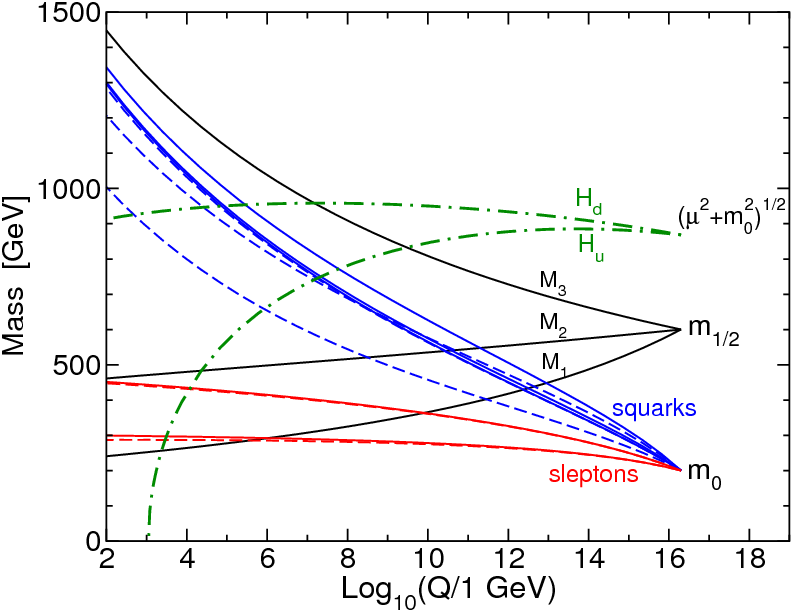
\includegraphics[width=0.6\textwidth]{figures/MSSMrun.png}
  \end{tabular}
  \caption{Evolution of scalar and gaugino mass parameters in the MSSM with mSUGRA boundary conditions imposed at $Q_0 = 2 \times 10^{16}$\gev. The parameter $\mu^2 + m^2_{H_{u}}$ runs negative, provoking electroweak symmetry breaking. Taken from~\cite{Martin:1997ns}.}
  \label{fig:MSSMrun}
\end{figure}
As discussed above, SUSY particles are expected to have the same mass as their corresponding SM partner particle. However, none of such particles has been observed so far which implies that supersymmetry in fact must be broken and that sparticles are actually heavier than the SM counterparts. If SUSY is expected to provide a solution to the hierarchy problem, the mass difference to the SM particles should consequently not be too large and the characteristic mass scale needs to be around 1\tev~\cite{Martin:1997ns}. \\
Typically, SUSY breaking is introduced such that so-called \textit{soft breaking} terms, \ie of positive mass dimension, are added to the theory in addition to the terms determining the gauge and Yukawa couplings. The SUSY breaking is assumed to take place in a hidden sector which does not couple directly to the visible sector represented by the supermultiplets. In this case, no specific breaking mechanism must be assumed, but only a mechanism to describe the mediation of the supersymmetry breaking from the hidden to the visible sector. In total, the MSSM including soft SUSY breaking features several new phases, mixing angles and masses which add another 105 free parameters to the already existing parameters of the SM~\cite{Dimopoulos:1995ju}.  \\
Two SUSY breaking scenarios, that are often studied, are either based on gravity-mediated or gauge-mediated interactions and known as \textit{minimal supergravity} (mSUGRA)~\cite{Chamseddine:1982jx, AlvarezGaume:1983gj} or \textit{constrained MSSM} (CMSSM)~\cite{Kane:1993td, Baer:2002gm} and \textit{gauge-mediated supersymmetry breaking} (GMSB)~\cite{Dine:1981gu, AlvarezGaume:1981wy}. Assuming a specific breaking scenario usually allows to drastically reduce the number of free parameters in the theory and determines the phenomenology of the respective model. In case of mSUGRA/CMSSM, the whole model can be described by five parameters, which are the common scalar mass $m_0$ and the common mass of the gauginos and higgsinos $m_{1/2}$ at the GUT scale, the common trilinear coupling $A_0$, $\mathrm{tan} \, \beta = v_u/v_d$ and the sign of the higgsino mass parameter $\mu$. In Fig.~\ref{fig:MSSMrun} the evolution of the corresponding mass parameters to the electroweak scale are illustrated.  

\section{Searches for Supersymmetry and Current Constraints}
\label{sec:susy_status}
The appealing attributes of supersymmetry, which have been discussed above, initiated a couple of indirect and direct searches looking for hints of supersymmetric particles. Although no sign for SUSY has been observed in nature so far, several results have been used in order to constrain the allowed parameter space. This section gives a short introduction to general search strategies for supersymmetry with main focus on collider experiments and provides a short overview of the status of experimental results. Results of direct searches at the LHC discussed in this section are restricted to results from searches performed previous to the analysis presented in this thesis. Further discussion of the status of supersymmetry after LHC Run-I follows in Sec.~\ref{sec:susy_status}.  

\subsection{Indirect Constraints}
\label{subsec:susy_indirect}
The existence of supersymmetric particles can show up in manifold ways. For instance, higher-order contributions to SM processes could be induced from SUSY. Such contributions might impact for instance electroweak precision data, rare decays of B-mesons or the anomalous magnetic moment of the muon. However, global fits to electroweak precision data using several precision measurements of SM parameters and particle masses, like $m_W$ and $m_t$, together with theoretical calculations have found no evidence for any inconsistency of the SM only hypothesis so far~\cite{LEP-2, Erler:2012wz, Ciuchini:2013pca, Baak:2014ora}. Furthermore, precise measurements of rare processes in B meson decays, like $B_s^0 \rightarrow \mu^+ \mu^-$, are in good agreement with expectations from the SM~\cite{Chatrchyan:2013bka, Aaij:2013aka, CMS-PAS-BPH-13-007}. The most compelling difference between experimental results and SM prediction, is currently observed for the anomalous magnetic moment of the muon~\cite{Bennett:2006fi, Hagiwara:2011af, Agashe:2014kda}. Here, deviations at the level of $3.6\sigma$ occur. However, discussions about the accuracy of the SM calculation are ongoing~\cite{Davier:2010nc}. \\  
Further constraints arise from astrophysical and cosmological observations. These occur from direct~\cite{cerdeno2010direct} and indirect~\cite{Cirelli:2010xx} dark matter searches. Moreover, several observations suggest that a considerable amount of cold dark matter contributes to the composition of the universe~\cite{wmap, Ade:2013zuv}. Good candidates are weakly interacting massive particles (WIMPs), which could be the neutralino in SUSY models where it is the LSP. Consequently, also the observed cold dark relic density can put constraints on the MSSM parameter space assuming that it is caused by a neutralino LSP.      
\subsection{Direct Searches at Collider Experiments}
\label{subsec:susy_collider}
Although the exploitation of indirect searches for supersymmetry is very useful in order to constrain the allowed SUSY parameter space, the most stringent exclusion limits are derived from direct searches at collider experiments. Typically, searches for SUSY at colliders make use of the specific production and decay properties assuming $R$-parity conservation. As discussed in Sec.~\ref{sec:susy}, $R$-parity conservation implies that sparticles are only produced in pairs and decay via cascades into the lightest supersymmetric particle which is often assumed to be the lightest neutralino. This leaves the experiment undetected and manifests in missing energy or missing momentum. Such missing energy signatures are thus a key-feature of searches for supersymmetry in collider experiments. Depending on the type of supersymmetric particle produced, the missing energy can be accompanied by several leptons, photons or jets. Usually, searches are classified according to their targeted final state and aim at a specific kind of supersymmetric particle. If searches are designed to be sensitive to various types of particles and models, they are called \textit{inclusive} searches. \\  
Extensive searches resulting in the tightest exclusion limits in the pre-LHC era have been realised by the experiments performed at \hera, \lep and \tevatron:
\begin{description}
 \item \textbf{\hera:} At \hera, searches for $R$-parity conserving supersymmetric models have mainly targeted processes involving the production of a selectron and a squark. The dominant MSSM process at \hera is the production of a selectron and a squark via the exchange of a neutralino where $\tilde{e}$ and $\tilde{q}$ subsequently decay into any lighter gaugino and their respective SM partner. Thus, a distinct experimental signature is given by an electron, hadrons and missing energy and momentum. Since no excess of such events over the SM expectation has been observed, exclusion limits for the masses of the selectron and squark in the context of the MSSM have been derived. Depending on the specific assumptions made to contrain the MSSM parameter space, the excluded region extends to around 60--70\gev for squark masses and around 40\gev for the LSP mass~\cite{Aid:1996es, Breitweg:1998gk}. 
 \item \textbf{\lep:} At \lep, various searches for supersymmetry were performed targeting different species of supersymmetric particles. Scalar leptons and quarks are mainly pair-produced in the $s$-channel via $Z$ bosons and photons. In case of selectrons, also the $t$-channel exchange of neutralinos yields important contributions. Typically, the energy scale at \lep opens a parameter space where sparticles with quite high masses are produced such that they predominantly decay into the respective SM partner particles (except for the scalar top, since the top quark is too heavy) and the lightest neutralino. Furthermore, also cascade decays are possible. Typical final states contain missing energy and a pair of acoplanar leptons (jets) where the direction of the first lepton (jet) is not in the plane defined by the direction of the second lepton (jet) and the beam direction. Similarly, neutralinos and charginos are expected to be pair-produced via $Z/\gamma$ $s$-channel exchange or $t$-channel selectron or sneutrino exchange, respectively. Typically, charginos decay into $\tilde{\chi}_{1}^{0}l\nu$ or $\tilde{\chi}_{1}^{0} qq'$ while in neutralino pairs ($\tilde{\chi}_{1}^{0}\tilde{\chi}_{2}^{0}$) the $\tilde{\chi}_{2}^{0}$ decays into $\tilde{\chi}_{1}^{0} \nu \bar{\nu}, \tilde{\chi}_{1}^{0} l^+ l^-$ or $\tilde{\chi}_{1}^{0} qq'$. Hence, the final state in case of chargino production is characterized by missing energy accompanied by four jets, two jets and one lepton or only leptons, depending on the specific decay mode of the chargino while the most important signature for neutralino production are acoplanar pairs of jets or leptons coming along with large missing momentum. However, the exact decay topologies strongly depend on the particular mass spectrum of the supersymmetric particles so that the above mentioned topologies could also be accompanied by photons or manifest in multiple jets or leptons in cascade decays. \\
Interpretations of combined results from all four experiments in the mSUGRA model lead to exclusion limits showing that $m_{1/2}$ has to be greater than about 100--200\gev over a range of $m_{0}$ up to the\tev-region for specific fixed other parameters. The lower limit on the LSP mass is found to be around 50\gev~\cite{ALEPHSUSY, DELPHISUSY, L3SUSY, OPALSUSY, LEPLimits}. 
 \item \textbf{\tevatron:} The \tevatron accelerator made a further SUSY parameter space for searches accessible, as the centre of mass energy exceeded that of \hera and \lep by at least one order of magnitude. A rich program of supersymmetric searches was enabled covering various final states of different lepton, photon or jet multiplicities. Of special interest is the search for coloured sparticles like squarks and gluinos, as \tevatron is a hadron collider. The expected decay topologies are very similar to those at the LHC and thus discussed below. \\
Results from SUSY searches at the Tevatron have been interpreted in the context of mSUGRA and extended the LEP results in the parameter region of $m_{0} =$ 70--300\gev and $m_{1/2} =$ 125--165\gev. This allows to exclude gluinos below around 280--300\gev for all squark masses and squarks below $380$\gev independent of the gluino mass~\cite{CDFLimits, D0Limits, Abazov200934}. 
\end{description}
\begin{figure}[!tp]
  \centering 
  \begin{tabular}{cc}
    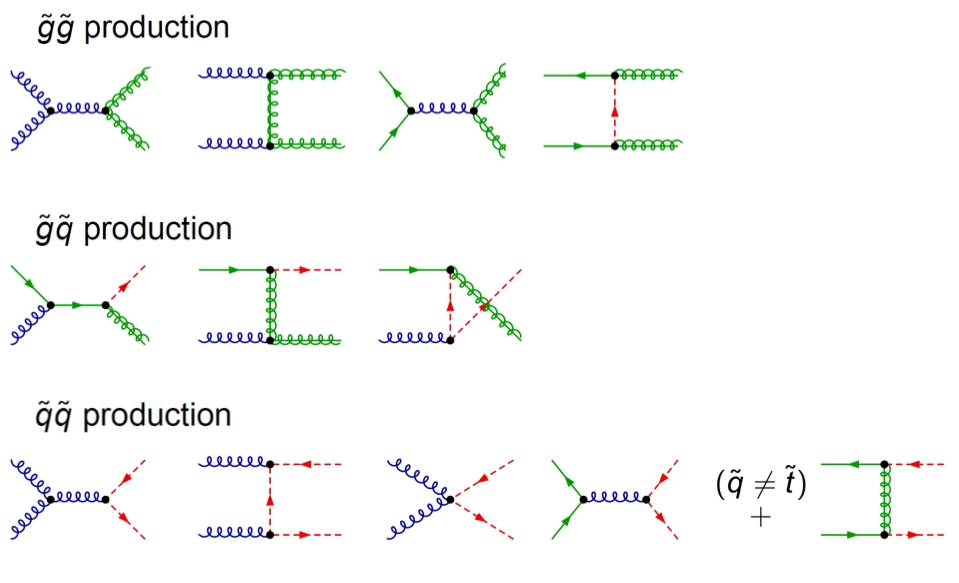
\includegraphics[width=0.75\textwidth]{figures/Susy_Feynman.jpg} 
  \end{tabular}
  \caption{Example diagrams for the production of supersymmetric particles in hadron collisions at parton level.}
  \label{fig:susy_feynman}
\end{figure}
The absence of SUSY-like signals at any collider experiment performed previously to the start of the LHC and exclusion limits at the order of a few hundred GeV on sparticle masses activated a variety of searches for supersymmetry at the LHC. It made already with a centre of mass energy of 7\tev an even larger SUSY parameter space accessible than the \tevatron. At the LHC, a variety of searches targeting the various different production and decay modes of supersymmetric partices are performed. In general, they can be classified into searches for electroweakinos, third generation sfermions and searches for squarks and gluinos. Of particular interest are searches for coloured particles, as the LHC is, as well as the \tevatron, a hadron collider. 
\\
At leading order sparticles in $R$-parity conserving models are predominantly produced in processes like~\cite{Kane:1982hw, Harrison:1982yi, Reya:1984yz, Dawson:1983fw, Baer:1985xz}
\begin{equation}
 pp \rightarrow \tilde{g}\tilde{g}, \tilde{g}\tilde{q}, \tilde{q}\tilde{q} \, .
\end{equation}
Some example diagrams for the production modes of such processes at parton level are shown in Fig.~\ref{fig:susy_feynman}. Typically, squarks are assumed to be mass-degenerate and refer to the partners of the light-flavour $(u, d, s, c)$ quarks with suppressed chiralities of the squarks $\tilde{q} = (\tilde{q}_L, \tilde{q}_R)$. Supersymmetric partners of the bottom and top quark are considered separately due to a potentially large mixing affecting the mass splitting.
\begin{figure}[!t]
  \centering
  % \makebox[\linewidth]{
  \begin{minipage}[c]{1.\textwidth}
    \begin{center}
      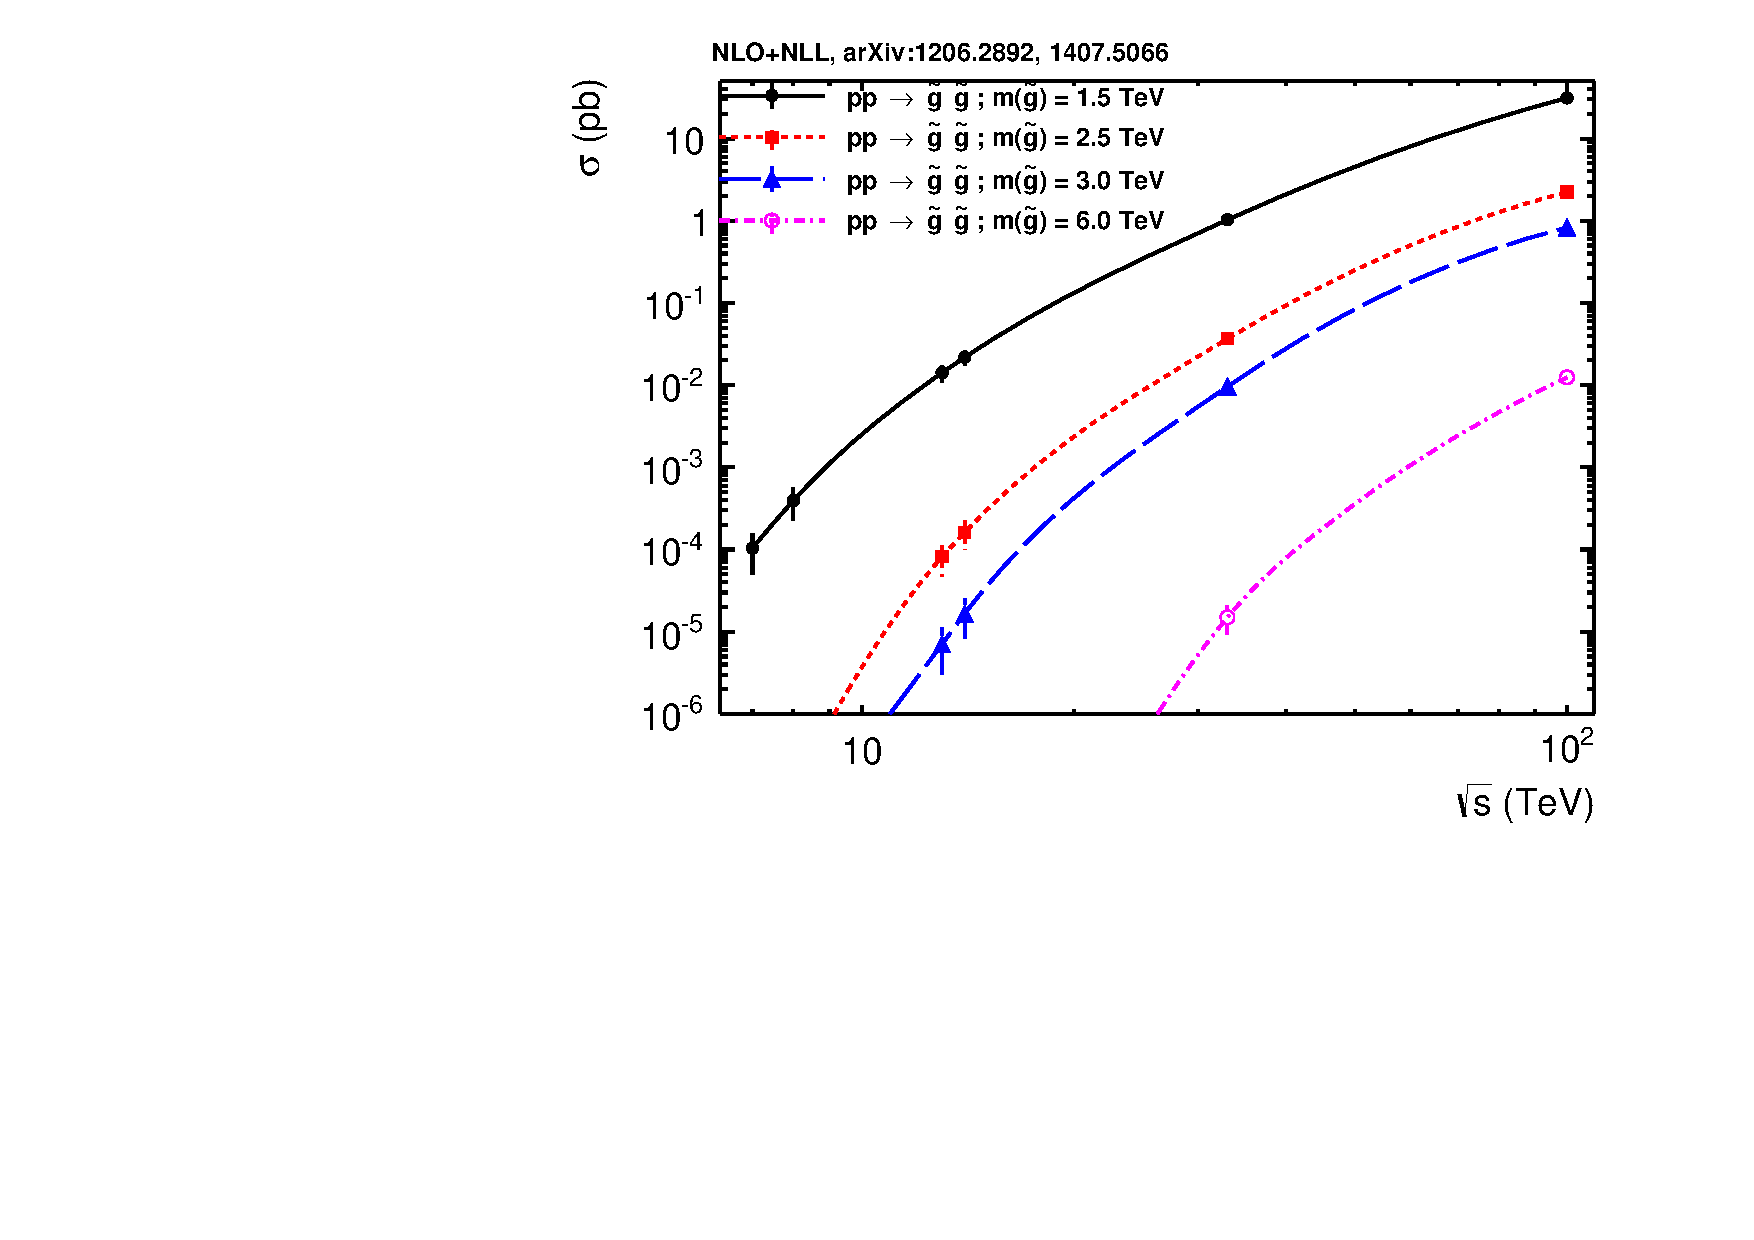
\includegraphics[width=0.495\textwidth]{figures/gluino_xsec.pdf}  
      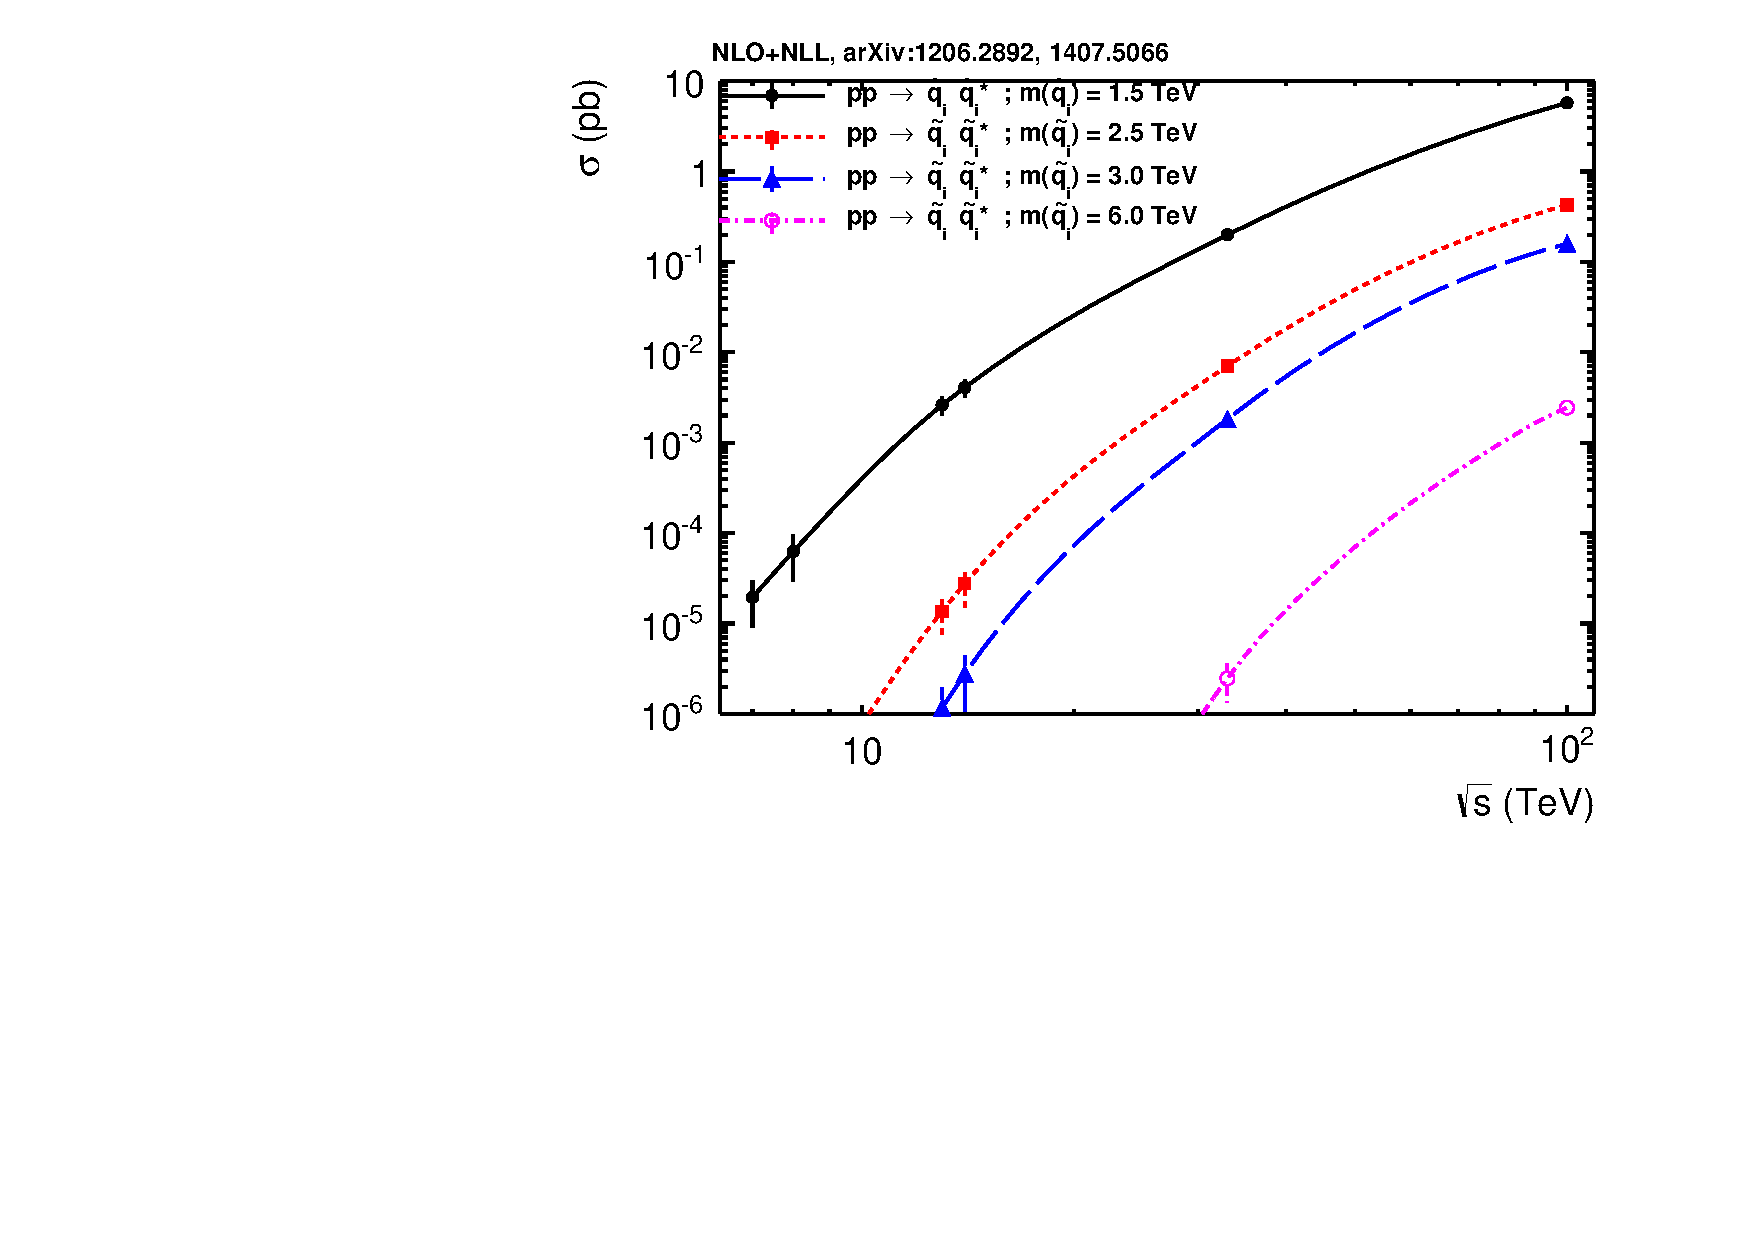
\includegraphics[width=0.495\textwidth]{figures/squark_xsec.pdf} \\
      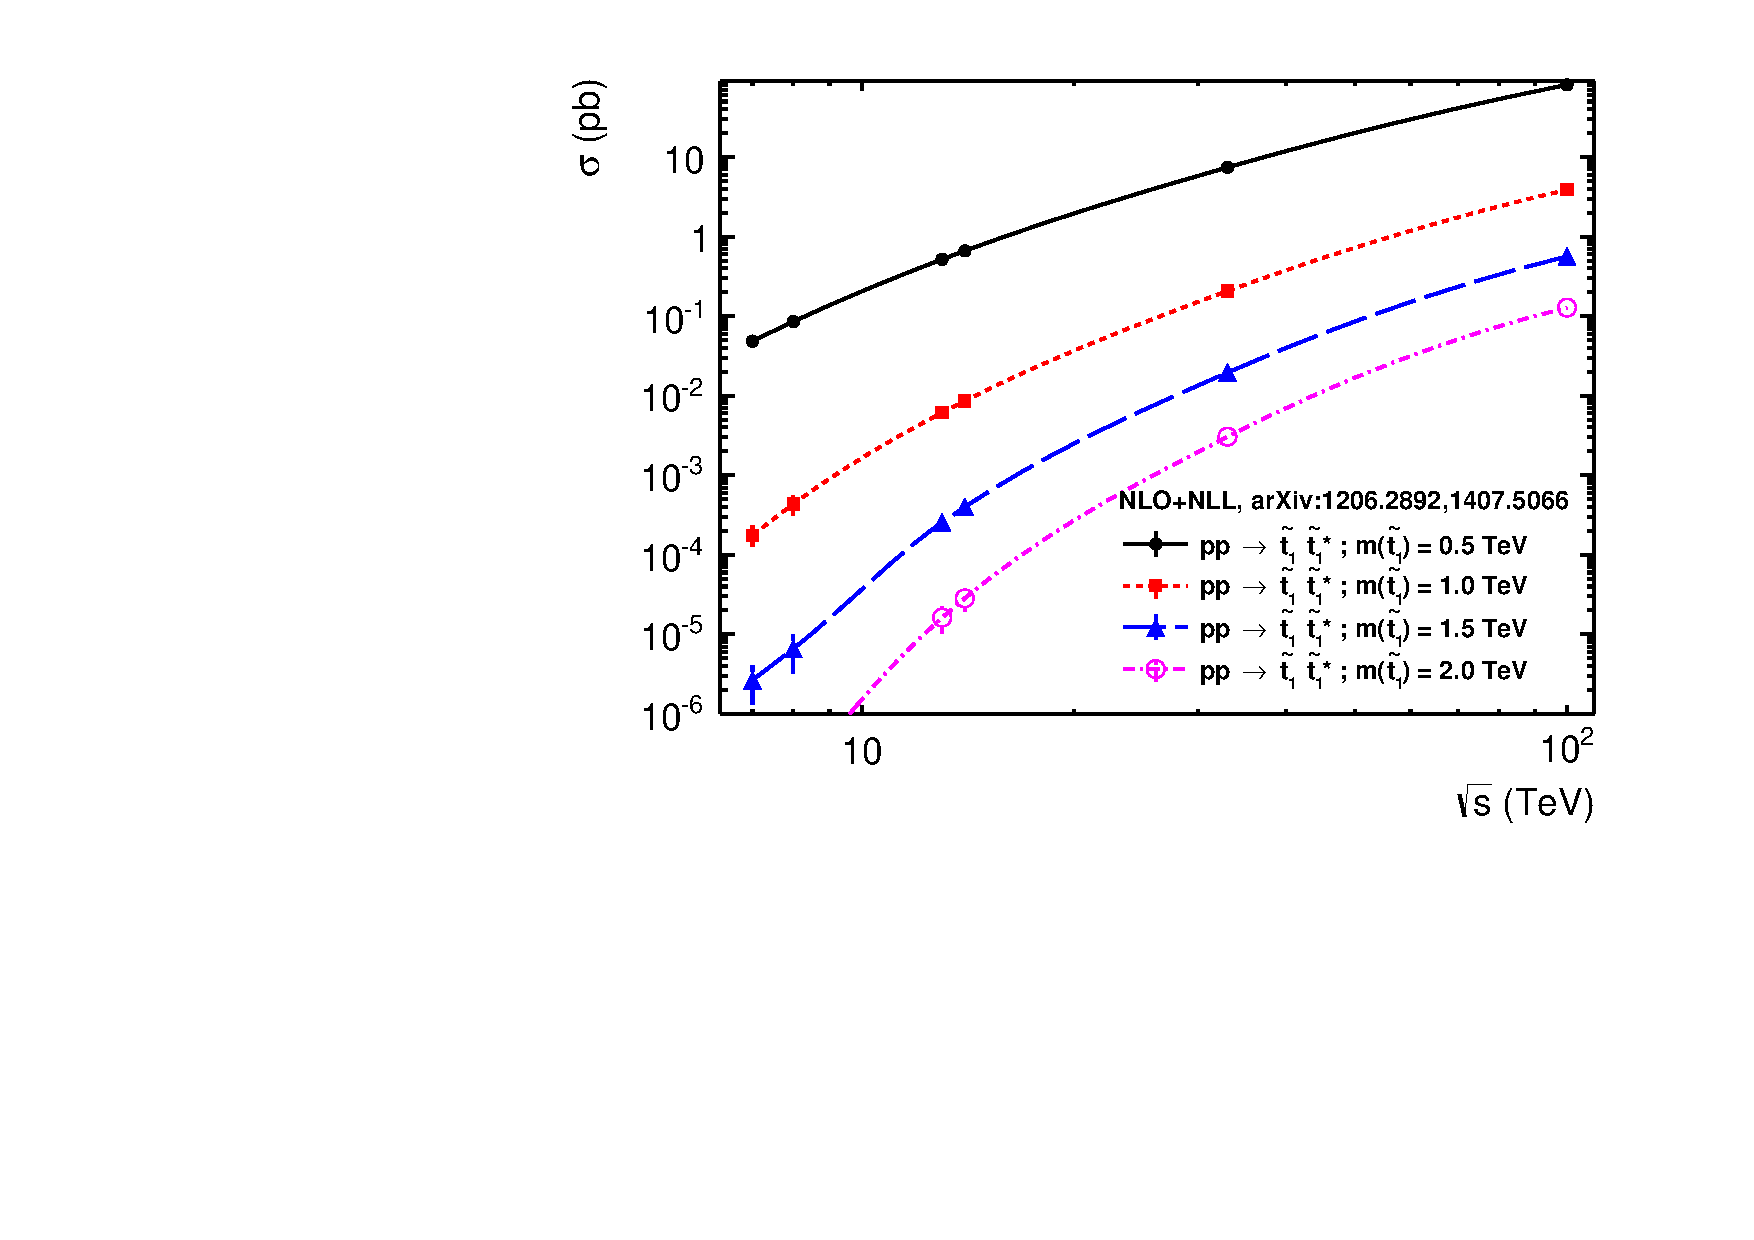
\includegraphics[width=0.495\textwidth]{figures/stop_xsec.pdf}
    \end{center}
  \end{minipage}
  \caption{SUSY production cross sections of processes $pp \rightarrow \tilde{g}\tilde{g}$ (\textit{top left}), $pp \rightarrow \tilde{q}\tilde{q}$ (\textit{top right}) and $pp \rightarrow \tilde{t}\tilde{t}$ (\textit{bottom}) displayed for different sparticle masses shown as function of the centre of mass energy~\cite{Kramer:2012bx, Borschensky:2014cia}.}
  \label{fig:susy_cross_sec}
\end{figure}
\\
Most recent SUSY cross section calculations consider higher order corrections caused, \eg by quark radiation or gluon loops, typically up to next-to-leading order (NLO). Production cross sections for the processes $pp \rightarrow \tilde{g}\tilde{g}$, $pp \rightarrow \tilde{q}\tilde{q}$ and $pp \rightarrow \tilde{t}\tilde{t}$ are illustrated in Fig.~\ref{fig:susy_cross_sec} for different sparticle masses as function of the centre of mass energy. For instance, for a gluino with a mass of 1.5\tev, the gluino pair-production cross section is expected to be at the order of $10^{-4}$\pb at $\sqrt{s} = 7$\tev. Typically, the relative size of the different channels depends on the respective squark and gluino masses as well as the energy of the collider. While for small masses of SUSY particles or large collider energies the cross sections of gluinos are dominant, squark-pair production (and also associated squark-gluino production) are favoured in case of large SUSY masses and low collider energies. \\
In addition to various different production channels, also the decay of supersymmetric particles offers a rich variety of different modes depending on the specific mass hierarchy. In Fig.~\ref{fig:susy_decay}, some example diagrams for possible decay modes of squarks and gluinos are illustrated. Here, the three-body decay of the gluinos in the upper two diagrams have to be understood as effective couplings. These occur in case squark masses are decoupled from the rest of the particle spectrum, \ie that their masses are significantly larger than that of the gluinos. While squarks are expected to decay preferrably into a quark and the LSP, gluinos predominantly decay into a quark pair and the LSP. In case of gluino decays, the quark pair can also be, for instance, a pair of top quarks representing the case of gluino-mediated stop production. In all such cases, a multijet final state accompanied by missing transverse momentum with no isolated leptons is expected as experimental signature\footnote{In general, final state topologies including leptons can occur as well, for instance in cascade decays or semi-leptonic decays of final state top quarks. However, since the analyses presented in this thesis concentrate on all-jet final states, final states including leptons are not discussed.}.  
\begin{figure}[!t]
  \centering
  % \makebox[\linewidth]{
  \begin{minipage}[c]{1.\textwidth}
    \begin{center}
      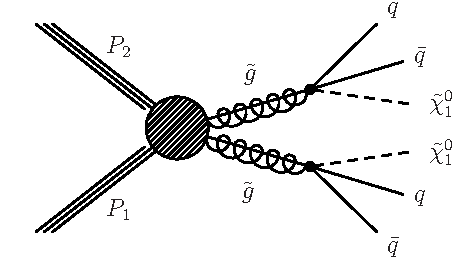
\includegraphics[width=0.49\textwidth]{figures/T1qqqq.pdf}  
      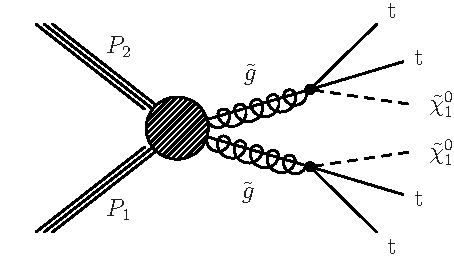
\includegraphics[width=0.49\textwidth]{figures/T1tttt_feyn.pdf} \\
      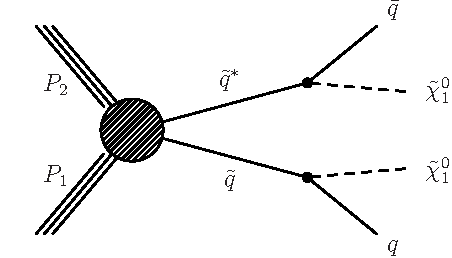
\includegraphics[width=0.49\textwidth]{figures/T2qq.pdf}
    \end{center}
  \end{minipage}
  \caption{Example diagrams of different SUSY decay channels showing $\tilde{g} \rightarrow q\bar{q} \tilde{\chi}_1^0$ (\textit{top left}), $\tilde{g} \rightarrow t\bar{t}\tilde{\chi}_1^0$ (\textit{top right}) and $\tilde{q} \rightarrow q\tilde{\chi}_1^0$ (\textit{bottom})~\cite{bib:CMS:PhysicsResultsSUS}.}
  \label{fig:susy_decay}
\end{figure}
\\
However, final states containing multiple jets accompanied by large values of missing transverse energy do not only arise from SUSY events, but are also realised for several SM processes. For any new physics search, such SM processes have to be considered as background, which is a crucial task in each SUSY analysis. In case of multijet + \met searches these are typically $\ZJets \rightarrow \nu \bar{\nu} + \mathrm{jets}$ events in which large genuine \met is caused by the neutrinos. This background is denoted \textit{invisible Z background} in this thesis. Furthermore, events with intrinsic missing energy stem from \WJets and \ttbar events. The top quark is the heaviest quark in the SM with a mass of $173.34 \pm 0.76$\gev~\cite{ATLAS:2014wva}. Since its lifetime is smaller than the hadronisation timescale, it decays before it forms colour-neutral hadrons. The decay takes place via the weak interaction and as denoted in Sec.~\ref{sec:sm}, the quark mixing is parametrized by the CKM-matrix. Since the corresponding matrix element $V_{\mathrm{tb}} \approx 1$, the top quark decays almost exclusively into a $W$ boson and a $b$ quark. Experimentally, the decay of the top-quark is characterized by the decay of the $W$ boson. In general, the $W$ boson can decay into a charged lepton and its corresponding neutrino or a pair of light quarks of the first two generations. Taking into account the three possible colour states for each quark pair, this gives rise to nine different $W$ decay modes and actually two thirds of top quark decays result exclusively in hadrons. However, since the targeted final state is assumed to contain a significant amount of missing energy only the semi-leptonic top quark decays relevantly contribute as background events. Thus, \WJets and \ttbar events featuring a decay containing an electron or muon that is not reconstructed, not isolated or falling out of the detector acceptance have to be considered as possible background. This source of background events is referred to as \textit{lost-lepton background}. Furthermore, also \WJets and \ttbar in which the lepton is a hadronically decaying $\tau$ lepton have to be accounted for. This background is known as \textit{hadronic-tau background}. Another source of background events is arising from QCD multijet events. Although these contain no intrinsic missing energy, severly mismeasured jets can give rise to large amounts of \met for instance because of instrumental effects or semi-leptonically decaying heavy-flavour quarks. This background process is denoted \textit{QCD background} in the following. Contributions from other SM processes are found to be negligible~\cite{springerlink:10.1007/JHEP08(2011)155, Chatrchyan:2012lia}. \\
\\
As soon as first collision data have been obtained at the LHC at a centre of mass energy of $\sqrt{s} = 7$\tev, searches for supersymmetry were carried out based on various final states. Like for previous collider experiments, however, no hints of new physics have been found and the results were interpreted in various SUSY models by setting exclusion limits. In Fig.~\ref{fig:CMSSM_7TeV}, interpretations of CMS searches for supersymmetry, based on various different hadronic and leptonic final states, are summarized in the context of the CMSSM. 
\begin{figure}[!tp]
  \centering 
  \begin{tabular}{cc}
    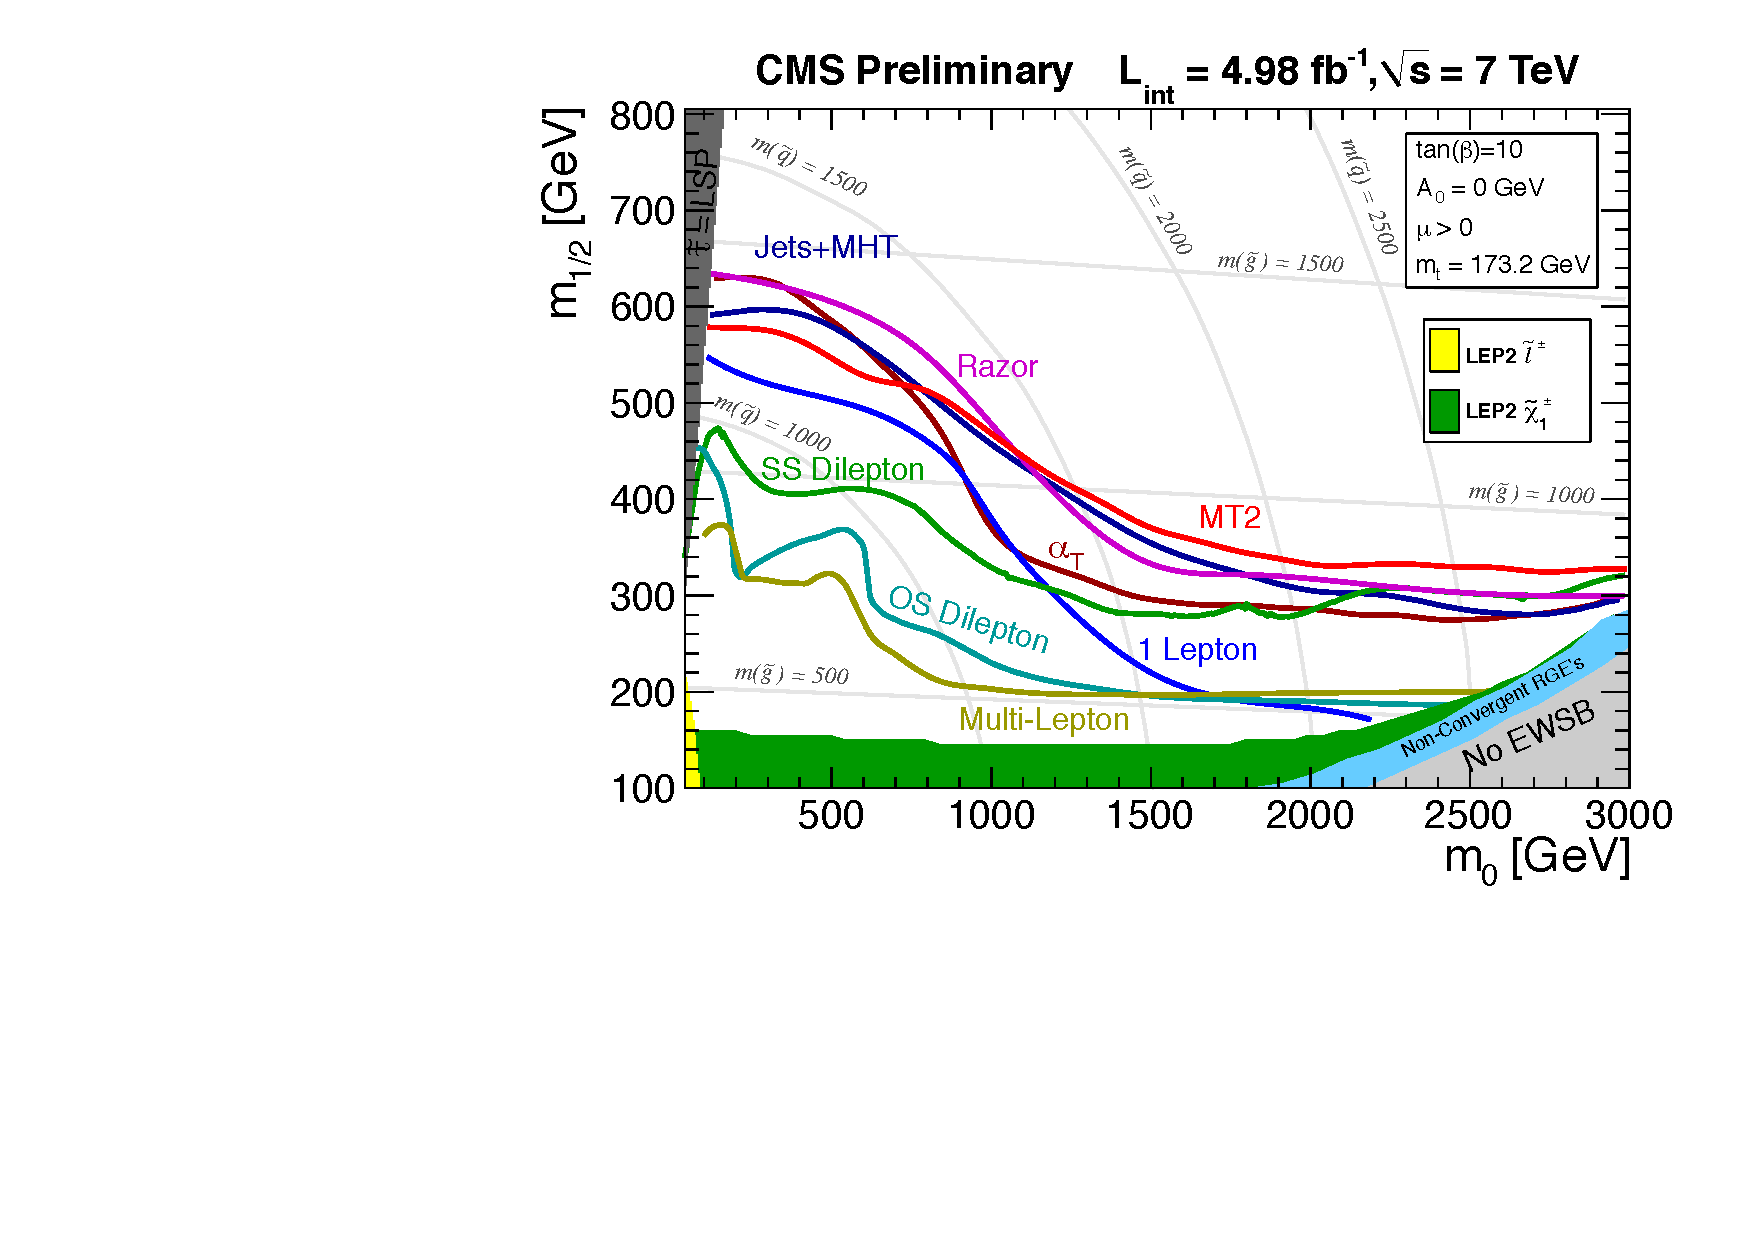
\includegraphics[width=0.7\textwidth]{figures/CMS_SUSY_2011Limits5fb_tanb10.pdf} 
  \end{tabular}
  \caption{Interpretation of searches for supersymmetry at the CMS experiment within the CMSSM. Shown are the 95\% CL exclusion limits in the $m_0$ and $m_{1/2}$ plane for various searches performed using different final state topologies~\cite{bib:CMS:PhysicsResultsSUS}.}
  \label{fig:CMSSM_7TeV}
\end{figure}
For comparison, also the exclusion curves from the LEP experiments are illustrated in the $m_0/m_{1/2}$-plane which have been widely exceeded already with those early searches performed at the LHC. In general, the exclusions in the CMSSM $m_0/m_{1/2}$-plane translate into constraints on the respective sparticle masses of around 1.3\tev in case of $m_{\tilde{g}} = m_{\tilde{q}}$ obtained from searches based on all-hadronic states as described above. However, interpreting search results only in the context of the CMSSM carries some risks. The simplified assumption of universal gaugino masses at the GUT scale does not allow all mass patterns and signatures that are in general possible within the MSSM. Thus, the CMSSM imposes for some SUSY topologies too strong constraints. \\
Thus, results of SUSY searches are, in addition to interpretations in the CMSSM, also interpreted in the context of \textit{simplified models}~\cite{ArkaniHamed:2007fw, Alwall:2008ag, Alwall:2008va, Chatrchyan:2013sza}. Since often, many SUSY models predict a similar phenomenology, simplified models do not rely on detailed descriptions of specific model parameters, but moreover characterize the dominant features of SUSY events that are common for several SUSY and SUSY-like models. Thus, the characterization of basic properties allows a comparison of search results to any (more complex) model and provides a suitable framework for reinterpretations of results from SUSY searches. A simplified model is described by a set of particles, their masses and a certain sequence of the particle production and decay. Typical benchmark scenarios are for instance those illustrated in Fig.~\ref{fig:susy_decay} in which the only free parameters are the two sparticle masses. The branching ratios of the pair-produced initial particles into the final state particles are assumed to be 100\%. Interpretations of SUSY searches at the CMS experiment within the context of these simplified models are illustrated in Fig.~\ref{fig:SMS_7TeV} for $\tilde{g} \rightarrow qq\tilde{\chi}^0$ and $\tilde{q} \rightarrow q \tilde{\chi}^0$. These illustrate the 95\% confidence level upper limit on the product of the cross section and branching fraction as function of the sparticles masses. Hence, the values of cross sections times branching ratio can be compared to any theoretical prediction in order to determine whether the specific model is compatible with data. The exclusion curves shown in Fig.~\ref{fig:SMS_7TeV} indicate that, in the context of these specific simplified models, gluinos with masses up to around 1\tev and light-flavour squarks around 800\gev are excluded in case of LSP masses up to around 100\gev. \\
However, interpretations in simplified models typically target only well-defined isolated SUSY topologies and thus do not account for all possible decay patterns in the MSSM. Consequently, also interpretations in more general models are desirable. One such example of a more generic SUSY model is the pMSSM~\cite{Djouadi:1998di}. The pMSSM is a 19-parameter realization of the MSSM and captures most of the features of general $R-$parity conserving SUSY models and covers a wide diversity of possible SUSY topologies. The MSSM is constrained by assuming that there is no new source of $CP$-violation, that no flavour changing neutral currents occur and that the first two sfermion generations are degenerate. Interpretations of CMS SUSY searches performed at $\sqrt{s} = 7$\tev within the pMSSM are published in~\cite{CMS-PAS-SUS-12-030}. A discussion of updated results follows in Sec.~\ref{sec:susy_status}.
\begin{figure}[!tp]
  \centering 
  \begin{tabular}{cc}
    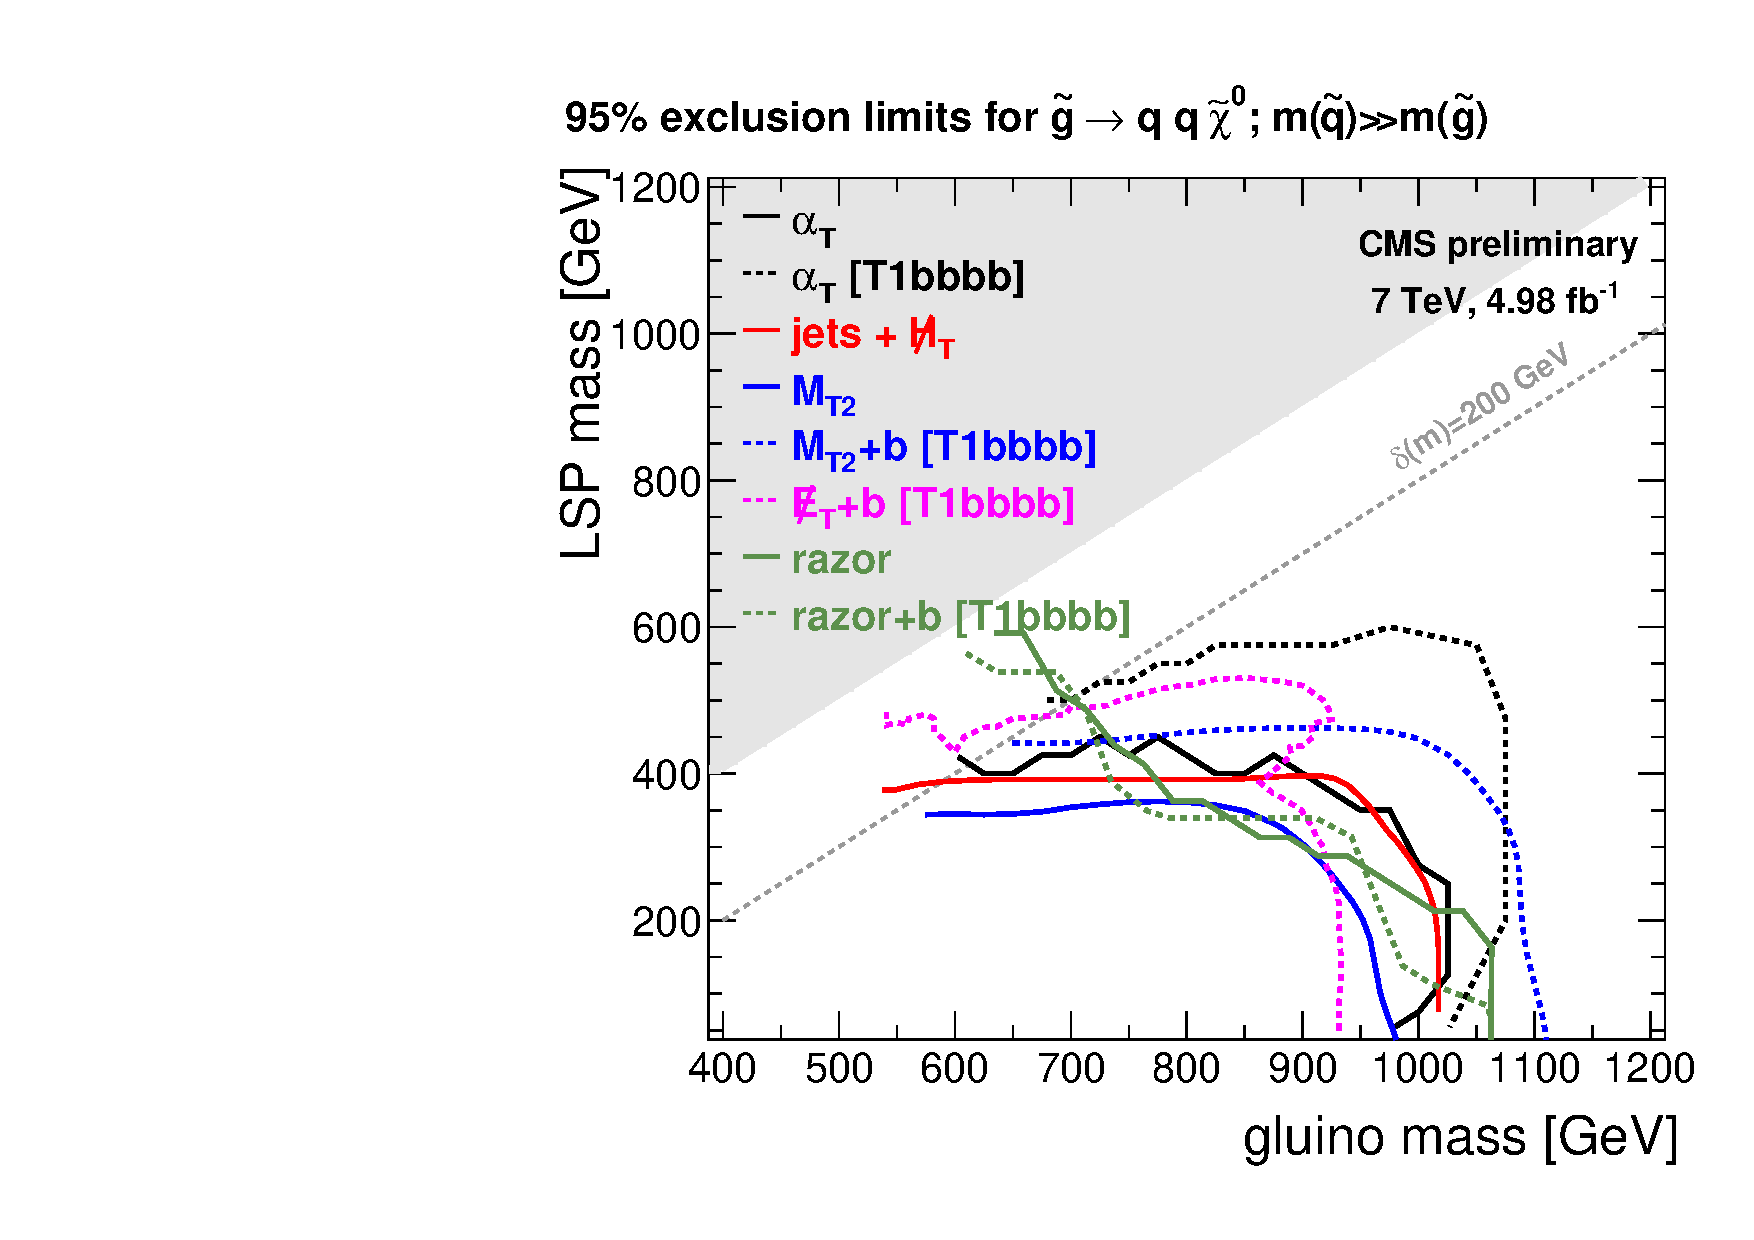
\includegraphics[width=0.49\textwidth]{figures/T1_7TeV.pdf} &
    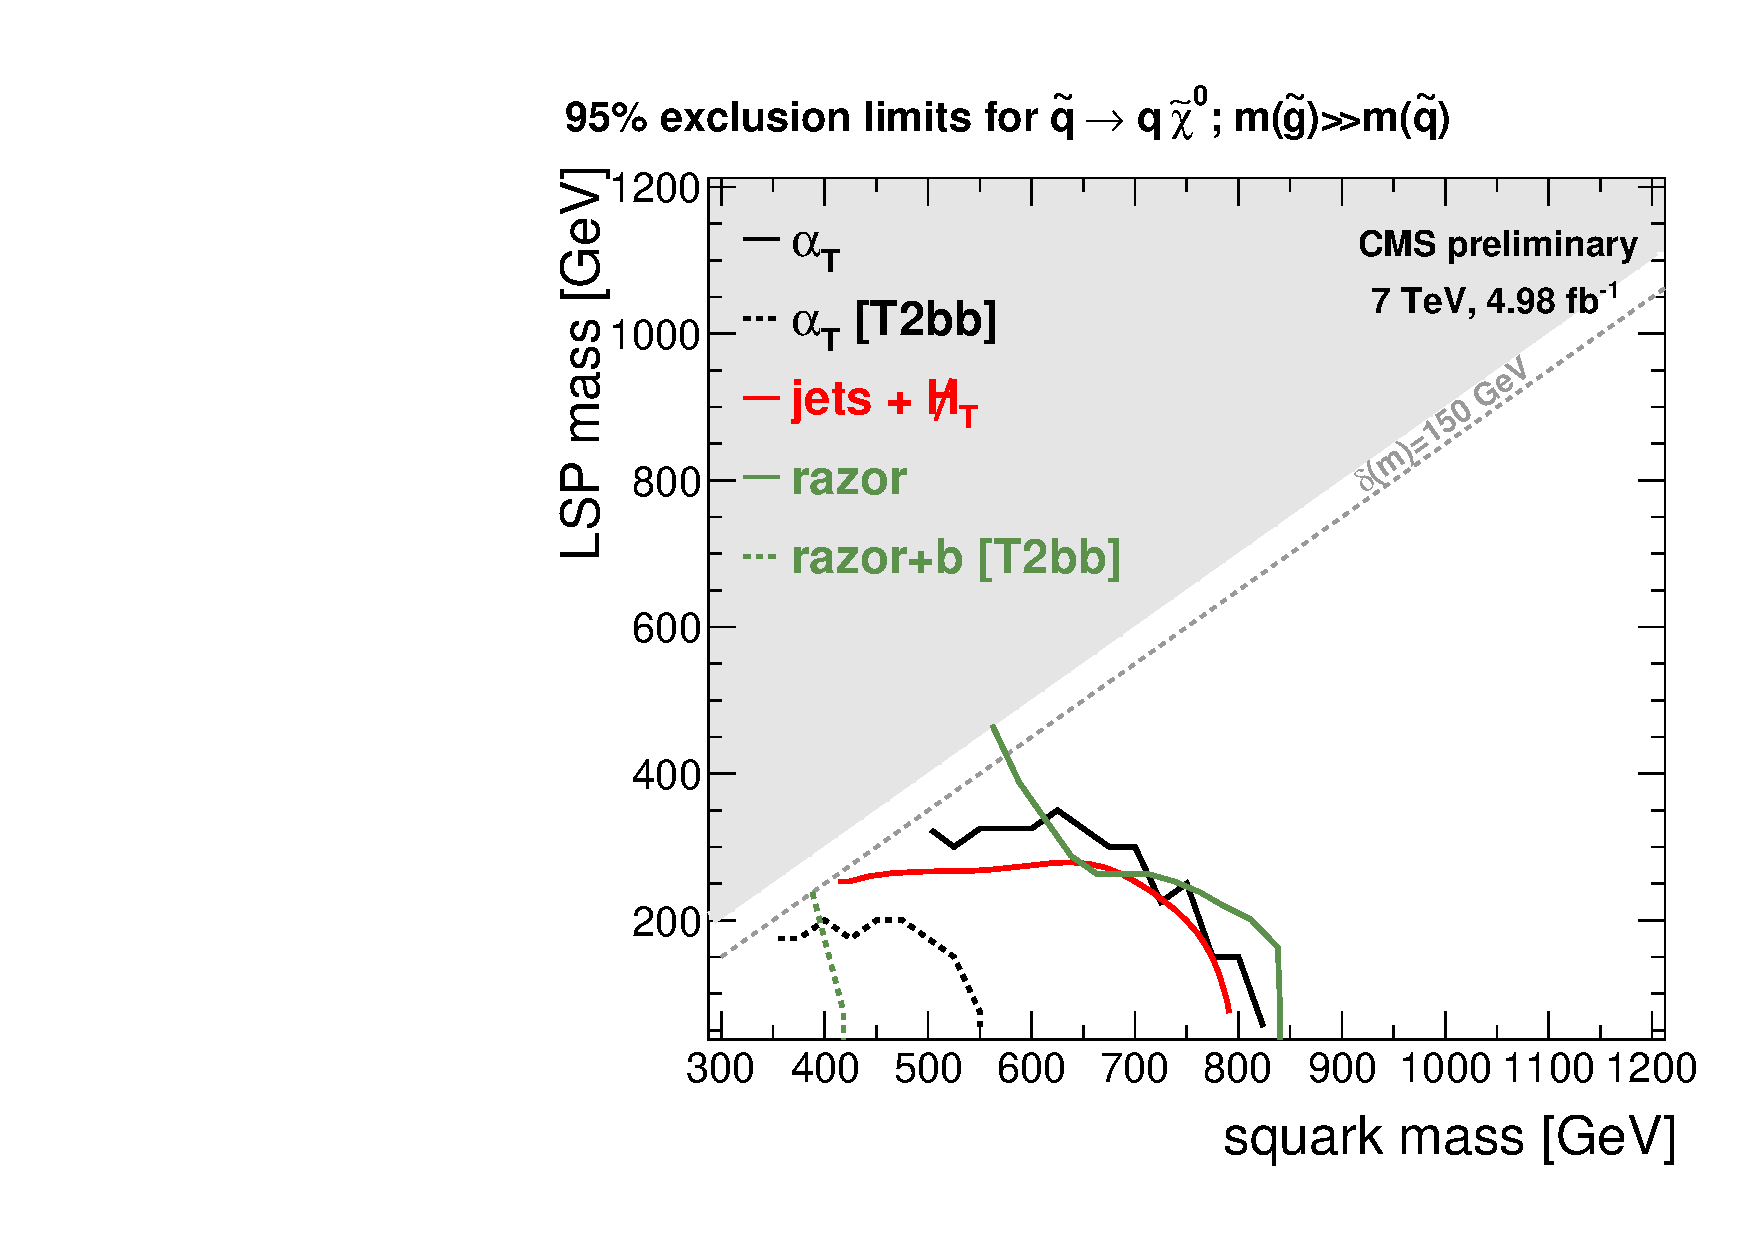
\includegraphics[width=0.49\textwidth]{figures/T2_7TeV.pdf}
  \end{tabular}
  \caption{Interpretation of searches for supersymmetry at the CMS experiment with simplified models in $\tilde{g} \rightarrow qq\tilde{\chi}^0$ (\textit{left}) and $\tilde{q} \rightarrow q \tilde{\chi}^0$ (\textit{right}) topologies. Shown are the 95\% CL upper limits on the produced particle and LSP masses. The grey area represents the region where the respective decay mode is forbidden~\cite{Chatrchyan:2013sza}.}
  \label{fig:SMS_7TeV}
\end{figure}
\\
Although the SUSY parameter space has been investigated already extensively with the LHC data obtained at $\sqrt{s} = 7$\tev and exclusion limits on sparticle masses enter the TeV range, searches for supersymmetry stay a very important field within the CMS experiment also for $\sqrt{s} = 8$\tev. As seen already in Fig.~\ref{fig:susy_cross_sec}, production cross sections are expected to largely increase for increasing centre of mass energies. In particular, gluino and light-flavour squark production cross sections profit a lot from the collider energy increase, such that a new parameter space is accessible. Thus, in particular searches for those sparticles based on final states containing several hard jets and high values of missing transverse momentum are of major interest for analyses of the LHC $\sqrt{s} = 8$\tev data.   






